\documentclass[11pt]{article}
\usepackage[margin=1in]{geometry}
\usepackage[T1]{fontenc}
\usepackage{lmodern}
\usepackage{amsmath,amssymb}
\usepackage{booktabs}
\usepackage{graphicx}
\usepackage{xcolor}
\usepackage[numbers,sort&compress]{natbib}
\usepackage[colorlinks=true,linkcolor=blue!50!black,citecolor=blue!50!black,urlcolor=blue!50!black]{hyperref}
\usepackage{url}
\usepackage{enumitem}
\setlist{nosep,leftmargin=*}
\newcommand{\PENDING}[1]{\textbf{\textcolor{red!70!black}{[PENDING: #1]}}}
\newcommand{\NOTE}[1]{\textcolor{orange!80!black}{[Author note: #1]}}

\title{Skill Cartridges: Composable, Hot-Swappable Deletion Masks\\for Small Language Models}
\author{Austin Dixson\\Independent researcher\\\texttt{austintdixson@gmail.com}}
\date{Preprint, November 11, 2026}

\begin{document}
\sloppy
\maketitle

\begin{abstract}
Deletion Tuning \citep{lu2026deleting} adapts a pretrained language model by learning a binary mask that sets a small fraction of its MLP gate-projection weights to zero, and nothing else. We treat these masks as \emph{skill cartridges}: small files that are applied to, and removed from, one frozen base model at request time. Using the authors' method and released code as our base, we test how far the idea goes on single-GPU budgets. A ToolAlpaca cartridge for Qwen3.5-9B raises exact-match accuracy from 42 to $69.3 \pm 1.5$ of 97 items across three training seeds (each seed $p \le 3\times10^{-8}$, exact McNemar test). The same recipe on a 27B model reaches 65. Masks from different seeds share 12 to 13 times more deleted weights than chance would predict, and 777,898 weights are deleted by all three seeds, where 489 would be expected. On a 4-bit MLX build of the 9B running on an Apple-silicon Mac, all three seeds keep the gain: from a shared base of 38 of 97 (identical per item across repeats), the nearest-zero form scores 66, 66 and 61, and requantize scores 66, 65 and 62, with at most one item lost per seed. Swapping in a prepared cartridge takes 0.04\,ms, and ejecting it restores the base weights bit for bit. The union of two published Qwen2.5-7B masks keeps 85\% of the tool-use gain and 97.9\% of the science gain. The same union operator on two cartridges we trained for Qwen3.5-9B keeps 87.5\% and 90.8\%. The method also works on LiquidAI's LFM3-1.7B, a hybrid convolution and attention model (11 to 59 of 97). A cartridge trained on synthetic latest-value recall lifts the 9B from 89 to 200 of 200 and from 8 to 100 of 100 on a longer held-out variant. A code cartridge trained on MBPP reference solutions made the model worse, and we report it in full. On a 4-bit 27B build, four general-knowledge tasks drop by a mean of 0.76 points on a 34\% subset, and no single task drops by more than 1.2 points. One 9B training run costs about \$0.60.\footnote{Code: \url{https://github.com/austindixson/skill-cartridges}. Cartridges: \url{https://huggingface.co/austindixson/skill-cartridges}.}
\end{abstract}

\section{Introduction}

Lu et al.\ \citep{lu2026deleting} showed that a large language model can learn new tasks when post-training is restricted to deleting pretrained weights. Their method, Deletion Tuning, learns one logit per gate-projection weight, anneals a sigmoid of those logits into a hard keep/delete decision, and deploys the result as a one-bit mask. Across GRPO, supervised fine-tuning and on-policy self-distillation it matches full fine-tuning at the largest scale they test, the masks are hundreds to thousands of times smaller than a fine-tuned checkpoint, and the model forgets less. They also point out that the masks are cheap to switch, and in their limitations section they suggest that masks for different tasks ``might also be combined, for example by taking their union.''

This paper takes those observations as a starting point and asks what is needed to run a small local model as one frozen set of weights plus a shelf of masks, one per skill, chosen per request. We call each mask a \emph{skill cartridge}. The term is ours and describes a deployment pattern; the training method is Deletion Tuning as published. Whether the pattern works depends on questions the original paper did not set out to answer: whether a small model with a cartridge can stand in for a larger one, whether the masks are reproducible across seeds, whether they survive the 4-bit quantization that small machines need, whether two cartridges can be active at once, and whether the method carries over to other architectures and skills.

\paragraph{What comes from prior work.} The training objective, the sigmoid relaxation and sharpness schedule, the Wanda-based initialization, the sparse-weight regularizer, the mask file format and the ToolAlpaca and Science evaluation settings are those of Lu et al.\ \citep{lu2026deleting}, who in turn build on MaskLLM \citep{fang2024maskllm}, Wanda \citep{sun2023wanda} and the SDFT task setup of Shenfeld et al.\ \citep{shenfeld2026sdft}. The two Qwen2.5-7B masks used in our stacking test are the authors' published masks. Our training script is a modified copy of their \texttt{train\_sft.py} at a pinned commit (Appendix~\ref{app:repro}).

\paragraph{What is new here.} All of the following were measured by us on November 10--11, 2026:
\begin{enumerate}
\item \textbf{A smaller model with a cartridge matches a larger one with a cartridge.} A Qwen3.5-9B ToolAlpaca cartridge scores $69.3 \pm 1.5$ of 97 against 65 for a cartridge trained with the same recipe on a 27B model, and against 42 for both base models (\S\ref{sec:size}).
\item \textbf{Replication across seeds and a mask-overlap analysis.} All three 9B seeds are individually significant, and their deleted sets overlap far above chance, with a shared core of 777,898 weights (\S\ref{sec:seeds}).
\item \textbf{4-bit retention with a live toggle on Apple silicon.} Two ways of applying a mask to an affine 4-bit model keep the gain on all three 9B ToolAlpaca seeds. We report apply and eject timings and verify exact restoration (\S\ref{sec:quant}).
\item \textbf{Union stacking.} We test the union operator that Lu et al.\ proposed as future work, on their two published 7B masks and on two cartridges we trained on the 9B (\S\ref{sec:stack}).
\item \textbf{A second architecture.} A cartridge on LiquidAI LFM3-1.7B, whose layers mix gated short convolutions with attention (\S\ref{sec:lfm}).
\item \textbf{A recall cartridge.} A cartridge for latest-value key--value recall that reaches ceiling and transfers to a longer held-out format (\S\ref{sec:memory}).
\item \textbf{A negative result for code.} An MBPP-trained cartridge lowered MBPP and HumanEval accuracy (\S\ref{sec:code}).
\item \textbf{Forgetting, perplexity and KL on the 27B cartridge.} Four off-task benchmarks drop by a mean of 0.76 points on a 34\% subset; WikiText-2 perplexity does not rise (\S\ref{sec:forget}).
\item \textbf{Low cost.} Every cartridge in this paper was trained on one rented GPU; a 9B run takes about 13 minutes and \$0.60 (\S\ref{sec:cost}).
\end{enumerate}

\section{Background: Deletion Tuning}
\label{sec:bg}

We summarize the method of \citep{lu2026deleting}. For a target weight matrix $W \in \mathbb{R}^{d_\text{out}\times d_\text{in}}$ (here every MLP gate projection) a logit matrix $G$ of the same shape is trained while all pretrained weights stay frozen. During training the layer uses
\begin{equation}
\widetilde{W}(t) = W \odot \sigma\big(\alpha(t)\,G\big), \qquad \alpha(t) = \alpha_\text{start} + \tfrac{t}{T}(\alpha_\text{end}-\alpha_\text{start}),
\end{equation}
and at deployment the hard mask $\widehat{W} = W \odot \mathbf{1}[G>0]$. Logits are initialized from Wanda scores $s_{ij} = |W_{ij}|\,\lVert X_j \rVert_2$ \citep{sun2023wanda}: weights in the bottom $\eta$ quantile receive logits drawn near $-0.03$ and the rest near $+0.03$. The SFT loss is the token-level negative log-likelihood of reference answers plus a MaskLLM-style regularizer $-\lambda \lVert \widetilde{W} \rVert_2^2$ \citep{fang2024maskllm}. No sparsity target is set. The deployed mask is bit-packed and zstd-compressed.

\section{Skill cartridges}
\label{sec:cartridges}

A \emph{cartridge} is a Deletion Tuning hard mask $M \in \{0,1\}^{N}$ over the $N$ gate-projection weights of a specific base checkpoint, stored in the upstream format (per layer: shape and zstd-compressed \texttt{np.packbits} of the keep mask, bit 1 = keep). We use $D(M)$ for its deleted set.

\paragraph{Composition.} Because a cartridge can only delete, two cartridges compose by set operations on deleted sets. The \emph{union} $D(M_1)\cup D(M_2)$ deletes every weight either cartridge deletes, and is the natural ``both skills on'' operator. The \emph{intersection} $D(M_1)\cap D(M_2)$ serves as a control. Composition is order-independent and needs no training.

\paragraph{Applying a cartridge to a 4-bit model.} Affine group quantization as implemented in MLX \citep{mlx2023} stores, per group of 64 input columns of a row, a scale $s$ and bias $b$, and per weight a 4-bit code $q$, with dequantized value $sq+b$. Zero is generally not representable. We compare two forms:
\begin{itemize}
\item \textbf{Nearest-zero.} Keep $s$, $b$ and all kept codes; replace each deleted weight's code with the code $q^\star = \arg\min_q |sq+b|$ under MLX's own dequantization. No kept weight changes. This form can be applied live to an already quantized model.
\item \textbf{Requantize.} Dequantize the layer, zero the deleted weights, and quantize again. Deleted weights become exactly zero more often, but scales, biases and many kept codes change.
\end{itemize}
On the Qwen3.5-9B 4-bit build with the seed-1 mask (10,702,823 deleted weights), nearest-zero lands 7,459,823 deleted weights exactly on 0 and changes no kept code; requantize lands 6,344,744 exactly on 0 and changes the dequantized value of 239,560,390 kept weights, because bf16 dequantize-then-quantize is not idempotent.

\paragraph{Live toggle.} The loader keeps a reference to the original arrays of every touched gate projection. \emph{Cold apply} computes the new arrays from the mask and swaps them in. \emph{Warm apply} swaps in arrays computed earlier. \emph{Eject} swaps the originals back. Every timed region ends with \texttt{mx.eval}.

\section{Experimental setup}
\label{sec:setup}

\paragraph{Models.} Qwen/Qwen3.5-9B (bf16, 32 layers, gate projection $12288\times4096$, $N = 1{,}610{,}612{,}736$); mlx-community/Qwen3.5-9B-MLX-4bit (affine, 4 bits, group size 64, converted from the same checkpoint; revision \texttt{938d8919}); a Qwen3.8-27B checkpoint, for which we trained our own masks; Qwen2.5-7B-Instruct \citep{qwen2024qwen25} with the two published masks; and LiquidAI/LFM3-1.7B \citep{liquid2026lfm3} (24 layers: 13 gated short convolutions, 5 sliding-window attention, 6 global attention), where the mask targets \texttt{feed\_forward.w1}, the gate of its gated MLP ($24 \times 7680 \times 2048 = 377{,}487{,}360$ weights). Qwen3.5-9B and the 27B model are different Qwen generations.

\paragraph{Tasks.}
\begin{itemize}
\item \textbf{ToolAlpaca} \citep{tang2023toolalpaca}, in the version prepared by Shenfeld et al.\ \citep{shenfeld2026sdft} (4,046 training examples, 97 test items), scored by exact match with their \texttt{eval\_tooluse.py} at commit \texttt{d7757321}.
\item \textbf{Science}: the SciKnowEval Chemistry L-3 subset \citep{feng2024sciknoweval} as prepared by \citep{shenfeld2026sdft} (507 test items), scored with their \texttt{eval\_science.py}.
\item \textbf{Latest-value recall} (ours). A prompt lists \texttt{name: value} assignment lines for 16 variables, each assigned a uniformly random 4 to 20 times in shuffled order (values 100 to 999), and asks for the current value of 4 of them. An item counts as correct only if all 4 values are right. Training uses 4,000 generated items; the 200 test items come from a fixed separate seed. A \emph{longer held-out} set (100 items) uses 32 variables assigned 20 to 40 times each, so it has twice the variables and roughly five times as many lines (about 7.6k versus 1.6k tokens). This format was never seen in training.
\item \textbf{Code}: training on the MBPP train, validation and prompt splits (474 problems, reference solutions as targets) \citep{austin2021mbpp}; evaluation by pass@1 under greedy decoding on the 500 MBPP test problems and on the 164 HumanEval problems \citep{chen2021humaneval}, with a 10\,s execution timeout.
\end{itemize}

\paragraph{Training.} All masks were trained with the same SFT recipe, which follows the upstream \texttt{scripts/train\_sft.sh} defaults: 400 optimizer steps, batch size 4, AdamW at learning rate $5\times10^{-4}$, no weight decay, gradient clipping at 1.0, $\eta = 1/2048$, Wanda prior strength 3, $(\alpha_\text{start},\alpha_\text{end}) = (100, 1000)$ and $\lambda = 10^{-5}$ decayed linearly to 0. Wanda calibration uses 256 training prompts. The loss is mean cross-entropy over answer tokens only. Maximum sequence length is 2048 (3072 for recall). Thinking mode is off. Training ran on one NVIDIA RTX PRO 6000 (96\,GB) through Hugging Face Jobs, except the 27B model, which used two. Our deviations from upstream \texttt{train\_sft.py} (building the mask once per optimizer step with the regularizer gradient added analytically, applying the LM head only at answer positions, fused AdamW, layer splitting over devices) change memory use and speed, not the objective; a unit test checks that the regularizer gradient matches.

\paragraph{Evaluation.} Greedy decoding with the model's chat template, at most 1024 new tokens for ToolAlpaca, 2048 for Science and 64 for recall. The 9B ToolAlpaca seed scores, and the LFM, recall and code numbers in bf16, come from each training job's own evaluation in PyTorch. The 9B Science score and the 9B stacking numbers were produced with MLX 0.32.4 and mlx-lm 0.32.2 on an Apple-silicon Mac (bf16); under that harness the 9B ToolAlpaca base scores 45 of 97, three above the PyTorch figure of 42. The 27B bf16 ToolAlpaca numbers come from the training job. The 4-bit ToolAlpaca numbers, the 7B stacking numbers, and the 27B forgetting, perplexity and KL numbers were produced with MLX 0.32.4 and mlx-lm 0.32.2 on Apple-silicon Macs. On the first eight ToolAlpaca items the MLX harness reproduced the PyTorch reference responses for the bf16 9B base exactly.

\paragraph{Statistics.} Base and cartridge are scored on the same items, so we report items gained and lost and an exact two-sided McNemar test \citep{mcnemar1947} (binomial test on the discordant pairs). For mask overlap we report Jaccard $J = |A\cap B|/|A\cup B|$ against the chance value $J_0 = pq/(p+q-pq)$ for independent deletions at densities $p$ and $q$, and observed intersections against the chance expectation $Npq$ (or $Npqr$ for three masks).

\section{Results}

\subsection{A 9B cartridge matches a 27B cartridge}
\label{sec:size}

\begin{figure}[t]
\centering
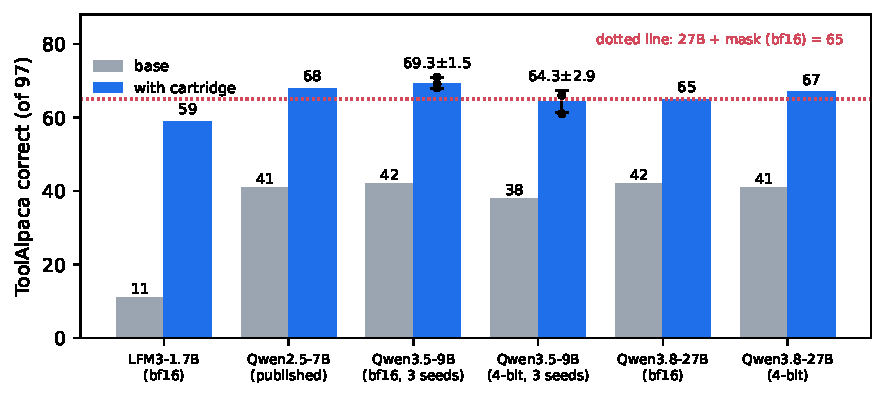
\includegraphics[width=\linewidth]{figures/fig1_toolalpaca.pdf}
\caption{ToolAlpaca exact match (of 97) with and without a cartridge. The 9B bf16 and 4-bit bars are means of three seeds (dots), with $\pm1$ s.d. The 7B mask is the published one from \citep{lu2026deleting}; all others were trained by us. 4-bit 9B numbers use the nearest-zero form.}
\label{fig:toolalpaca}
\end{figure}

\begin{table}[t]
\centering
\small
\begin{tabular}{lcccccc}
\toprule
Model & Precision & Base & Cartridge & Gained / lost & McNemar $p$ & Deleted \\
\midrule
Qwen3.5-9B, seed 1 & bf16 & 42 & 69 & 27 / 0 & $1.5\times10^{-8}$ & 0.6645\% \\
Qwen3.5-9B, seed 2 & bf16 & 42 & 71 & 30 / 1 & $3.0\times10^{-8}$ & 0.6799\% \\
Qwen3.5-9B, seed 3 & bf16 & 42 & 68 & 26 / 0 & $3.0\times10^{-8}$ & 0.6718\% \\
Qwen3.5-9B, seed 1 & MLX 4-bit & 38 & 66 & 28 / 0 & $7.5\times10^{-9}$ & 0.6645\% \\
Qwen3.5-9B, seed 2 & MLX 4-bit & 38 & 66 & 28 / 0 & $7.5\times10^{-9}$ & 0.6799\% \\
Qwen3.5-9B, seed 3 & MLX 4-bit & 38 & 61 & 24 / 1 & $1.5\times10^{-6}$ & 0.6718\% \\
Qwen3.8-27B (run 1) & bf16 & 42 & 65 & 29 / 6 & $1.2\times10^{-4}$ & 0.5037\% \\
Qwen3.8-27B (run 1) & MLX 4-bit & 41 & 67 & 28 / 2 & $8.7\times10^{-7}$ & 0.5037\% \\
LFM3-1.7B & bf16 & 11 & 59 & 48 / 0 & $7.1\times10^{-15}$ & 0.713\% \\
Qwen2.5-7B (published) & MLX bf16 & 41 & 68 & -- & -- & 0.783\% \\
\bottomrule
\end{tabular}
\caption{ToolAlpaca results (97 items). ``Deleted'' is the share of gate-projection weights the mask removes. 4-bit 9B rows are the nearest-zero form; requantize scores are in \S\ref{sec:quant}. The 4-bit 9B $p$ values are exact two-sided McNemar tests on the listed discordant pairs. A second 400-step 27B run deleted 0.6049\% and also scored 65; we use run 1 because it reaches the same score with fewer deletions (28,730,353 of 5,704,253,440 weights, 57.2\,MB).}
\label{tab:toolalpaca}
\end{table}

Table~\ref{tab:toolalpaca} and Figure~\ref{fig:toolalpaca} give the results. The 9B cartridge lifts the model from 42 to a three-seed mean of $69.33 \pm 1.53$ items ($71.5 \pm 1.6\%$). The 27B model with a cartridge trained by the same recipe scores 65; the 27B base scores 42, the same as the 9B base. The 9B with a cartridge is therefore at least as good as the 27B with one on this benchmark, with about a third of the parameters. We do not claim the 9B is significantly \emph{better}: the 4.3-item difference is between different models on 97 items and we have not run a paired test. The two models are also from different Qwen generations, so model generation and size are confounded.

The 9B gains are almost one-directional: across three seeds, 83 items flip from wrong to right and 1 flips from right to wrong. Each seed's 95\% interval on the gain lies between 18.6 and 39.2 percentage points.

\subsection{Seeds agree, and the masks share a core}
\label{sec:seeds}

\begin{figure}[t]
\centering
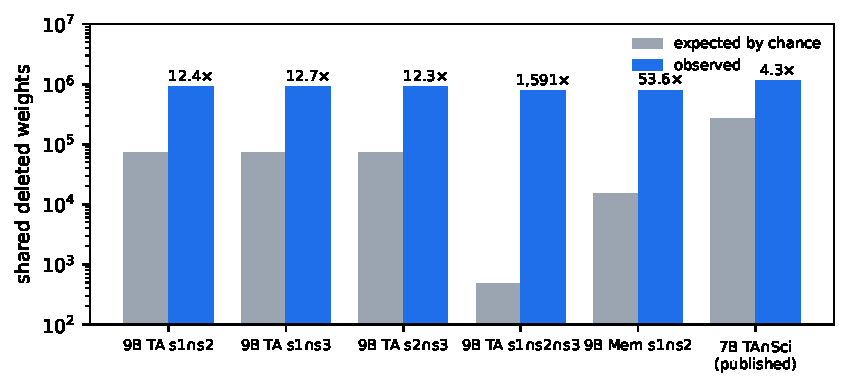
\includegraphics[width=\linewidth]{figures/fig2_overlap.pdf}
\caption{Observed shared deleted weights against the number expected if each mask deleted weights independently at its own density (log scale). Labels give observed/expected.}
\label{fig:overlap}
\end{figure}

\begin{table}[t]
\centering
\small
\begin{tabular}{lrrrrr}
\toprule
Pair (9B ToolAlpaca) & $|A\cap B|$ & Expected $Npq$ & $J$ & $J_0$ & $J/J_0$ \\
\midrule
seed 1 / seed 2 & 905,170 & 72,766 & 0.0436 & 0.00337 & 12.9 \\
seed 1 / seed 3 & 909,807 & 71,900 & 0.0441 & 0.00335 & 13.2 \\
seed 2 / seed 3 & 907,727 & 73,562 & 0.0435 & 0.00339 & 12.8 \\
all three & 777,898 & 489 & -- & -- & 1,591$\times$ (obs/exp) \\
\midrule
9B recall seed 1 / seed 2 & 797,965 & 14,882 & 0.0887 & -- & 53.6$\times$ (obs/exp) \\
7B ToolAlpaca / Science (published) & 1,140,547 & 263,271 & 0.0241 & 0.00546 & 4.4 \\
\bottomrule
\end{tabular}
\caption{Mask overlap. $N = 1{,}610{,}612{,}736$ for the 9B and $1{,}901{,}068{,}288$ for the 7B. The 9B seed rows were recomputed from the mask files for this paper and match the values recorded at training time.}
\label{tab:overlap}
\end{table}

The three seeds delete 10,702,823, 10,950,222 and 10,819,819 weights. Each pair shares about 0.9 million, 12 to 13 times the chance expectation (Table~\ref{tab:overlap}, Figure~\ref{fig:overlap}). Most of that is common to all three: 777,898 weights, or 86\% of a typical pairwise intersection, are deleted by every seed, against 489 expected by chance. The union of the three deleted sets is 30,528,058. So each run deletes a large seed-specific set plus a reproducible core of about 0.05\% of gate-projection weights. Per-layer deletion rates follow the same profile across seeds (Figure~\ref{fig:perlayer}), apart from seed 2's higher rate in layers 0 to 4.

Two cautions apply. First, part of the above-chance overlap may reflect weights that are cheap to delete in this model regardless of task. A preflight on the published 7B masks found that a GRPO math mask trained on a different Qwen2.5-7B checkpoint overlaps the ToolAlpaca mask 7.0 times above chance, which suggests such a task-independent component exists. We have not yet trained a matched random-task control for the 9B. Second, overlap is a statement about deleted sets; we have not shown that the core alone carries the gain.

\begin{figure}[t]
\centering
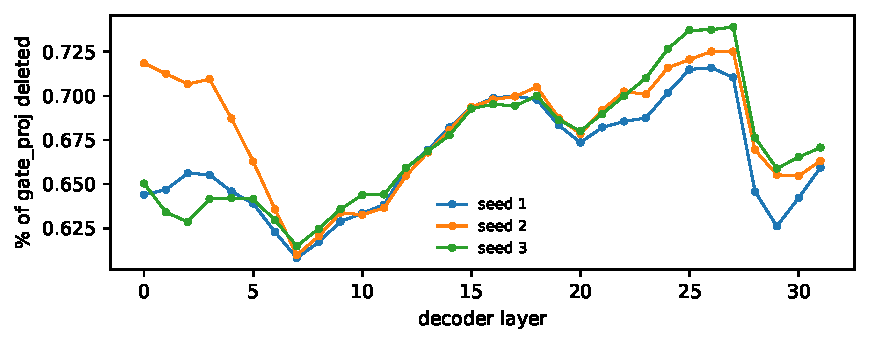
\includegraphics[width=\linewidth]{figures/fig4_per_layer.pdf}
\caption{Share of gate-projection weights deleted per decoder layer, Qwen3.5-9B ToolAlpaca, three seeds.}
\label{fig:perlayer}
\end{figure}

\subsection{Cartridges survive 4-bit quantization and toggle live}
\label{sec:quant}

On mlx-community/Qwen3.5-9B-MLX-4bit, the 4-bit base scores 38 of 97, four below bf16. That base is identical item by item across the three seed evaluations. All three seeds keep a large gain under both application forms (Table~\ref{tab:fourbit}):

\begin{table}[h]
\centering
\small
\begin{tabular}{lcccc}
\toprule
Seed & Nearest-zero & Gained / lost & Requantize & Gained / lost \\
\midrule
1 & 66 & 28 / 0 & 66 & 28 / 0 \\
2 & 66 & 28 / 0 & 65 & 27 / 0 \\
3 & 61 & 24 / 1 & 62 & 25 / 1 \\
\bottomrule
\end{tabular}
\caption{ToolAlpaca on the 4-bit 9B (97 items, shared base 38). Seed 3 lags the other two by a few items in both forms. Exact McNemar $p$ is $7.5\times10^{-9}$ for each 28/0 result, $1.5\times10^{-8}$ for 27/0, $1.5\times10^{-6}$ for 24/1 and $8.0\times10^{-7}$ for 25/1.}
\label{tab:fourbit}
\end{table}

For seed 1 the 4-bit gain (28 items) is slightly larger than the bf16 gain for the same mask (27). Nearest-zero is the form that can be toggled on a quantized model without touching kept weights, and it matches requantize here to within one item. On the 27B model, the run-1 cartridge on a 4-bit MLX build goes from 41 to 67 (28 gained, 2 lost, $p = 8.7\times10^{-7}$), against 42 to 65 in bf16.

Swap timings on the 4-bit 9B (nearest-zero form, all 32 gate projections, 10 repetitions): cold apply median 309\,ms, warm apply 0.04\,ms, eject 0.10\,ms. After eject, a host-side byte comparison of every touched weight, scale and bias array matched the originals, and the logits equalled the base model's in 20 of 20 checks. We also saw lower decode throughput with the requantized form in one batch-1 measurement (43.2 versus 65.6 tokens/s); a re-measurement was inconclusive, and we make no throughput claim.

\subsection{Union stacking}
\label{sec:stack}

\begin{figure}[t]
\centering
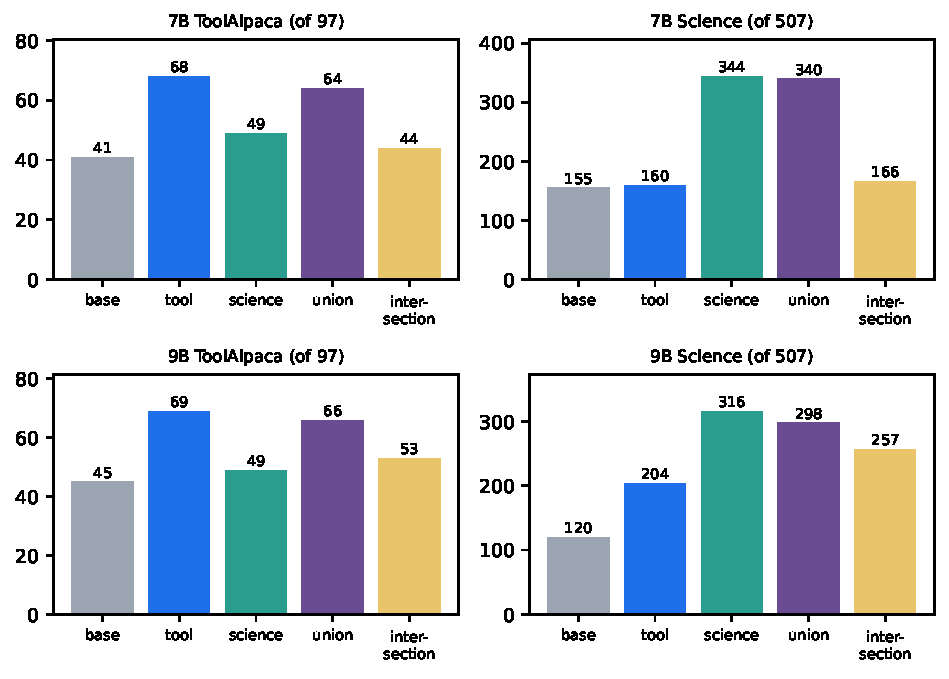
\includegraphics[width=\linewidth]{figures/fig3_stacking.pdf}
\caption{Union stacking. Top: the two published Qwen2.5-7B-Instruct masks of \citep{lu2026deleting} (MLX, bf16). Bottom: a ToolAlpaca cartridge and a Science cartridge we trained on Qwen3.5-9B (MLX, bf16). ``union'' deletes every weight that either mask deletes; ``intersection'' is the control that deletes only the shared weights.}
\label{fig:stack}
\end{figure}

Lu et al.\ suggest in their limitations section that masks for different tasks ``might also be combined, for example by taking their union.'' We test that operator on two pairs: the published Qwen2.5-7B-Instruct masks \citep{lu2026deleting}, and two cartridges we trained on Qwen3.5-9B. Figure~\ref{fig:stack} shows the scores.

\paragraph{Published 7B masks.} ToolAlpaca deletes 14,892,491 weights (0.783\%) and Science 33,607,213 (1.768\%). Their union deletes 47,359,157 weights (2.49\%), which is 97.6\% of the plain sum, so the two masks are close to disjoint ($J = 0.0241$, 4.4 times chance).
\begin{itemize}
\item ToolAlpaca: base 41, tool mask 68, science mask 49, union 64, intersection 44. The union keeps $(64-41)/(68-41) = 23/27 = 85\%$ of the tool gain.
\item Science: base 155, science mask 344, tool mask 160, union 340, intersection 166. The union keeps $(340-155)/(344-155) = 185/189 = 97.9\%$ of the science gain.
\end{itemize}
The intersection (1,140,547 weights) alone moves ToolAlpaca by only 3 items and Science by 11, so the shared weights do not carry either skill by themselves. Each mask applied alone barely helps or hurts the other task (tool mask on Science: $+5$; science mask on ToolAlpaca: $+8$). Our MLX numbers differ slightly from those reported in \citep{lu2026deleting} for the same masks (ToolAlpaca 68 versus 67 of 97; Science 344 versus about 358 of 507), which we attribute to the different inference stack.

\paragraph{9B cartridges.} We repeated the test with our seed-1 ToolAlpaca cartridge (10,702,823 deleted, 0.6645\%) and a Science cartridge trained for 330 of the planned 400 steps (8,696,798 deleted, 0.5400\%), scored with MLX in bf16. Their union deletes 16,530,526 weights (1.026\%) and their intersection 2,869,095 ($J = 0.1736$, against a chance Jaccard of $0.00299$, or 58 times chance). These two 9B masks overlap more than the published 7B pair; the union is 85.2\% of the plain sum.
\begin{itemize}
\item ToolAlpaca: base 45, tool mask 69 (24 gained, 0 lost), science mask 49 (9 gained, 5 lost), union 66 (22 gained, 1 lost, $p = 5.7\times10^{-6}$), intersection 53. The union keeps $(66-45)/(69-45) = 21/24 = 87.5\%$ of the tool gain.
\item Science (507 items): base 120, science mask 316 (211 gained, 15 lost, $p = 1.94\times10^{-45}$), tool mask 204 (113 gained, 29 lost), union 298 (199 gained, 21 lost, $p = 1.5\times10^{-37}$), intersection 257. The union keeps $(298-120)/(316-120) = 178/196 = 90.8\%$ of the science gain. Against the science mask alone the union is 18 items lower (46 gained, 64 lost), which is not significant ($p = 0.105$).
\end{itemize}
Unlike the 7B pair, the 9B tool mask alone already lifts Science substantially (120 to 204). The intersection also moves Science more than it does on the 7B (120 to 257, still well below the union and the solo mask). Both observations are consistent with the higher overlap, but we have not isolated a cause. The Science cartridge itself is a strong skill: 316 of 507, from a base of 120, even though training stopped early at 330 steps.

\subsection{A second architecture: LFM3-1.7B}
\label{sec:lfm}

LFM3-1.7B combines gated short convolutions with sliding-window and global attention \citep{liquid2026lfm3}; its MLP is gated, so the method applies to the gate matrix \texttt{w1} without changes. A ToolAlpaca cartridge (2,690,252 weights, 0.713\%, 4.98\,MB) lifts it from 11 to 59 of 97 (48 gained, 0 lost, $p = 7.1\times10^{-15}$) after a 290-second, \$0.22 job. Much of this gain is format compliance: the median response shrinks from 1,152 to 205 characters, and the base model often fails exact match by adding text around a correct call. We count this as a real gain under the benchmark's rules but not as evidence of better tool reasoning.

\subsection{A recall cartridge}
\label{sec:memory}

On latest-value recall (Section~\ref{sec:setup}) the 9B base gets all four values right on 89 of 200 test items. With the recall cartridge it gets 200 of 200 (111 gained, 0 lost, $p = 7.7\times10^{-34}$). On the longer held-out set it goes from 8 to 100 of 100 (92 gained, 0 lost, $p = 4.0\times10^{-28}$). A second seed replicated the result (90 to 200; 8 to 99), and the two recall masks (0.315\% and 0.293\% deleted) share 797,965 weights against 14,882 expected, 53.6 times chance. The cartridges are the smallest we trained, 10.8 and 10.1\,MB.

This is a narrow, synthetic task with a fixed format, and the longer set changes only scale. The result shows that deletion alone can switch on a precise state-tracking behaviour that the base model does poorly and that it extends to inputs about five times longer than those seen in training. It does not show better long-context memory in general; standard long-context benchmarks are future work.

\subsection{A negative result: code}
\label{sec:code}

A cartridge trained on MBPP reference solutions (12,678,451 weights, 0.787\%) made the 9B worse. MBPP test pass@1 fell from 349 to 293 of 500 (36 gained, 92 lost, $p = 7.9\times10^{-7}$) and HumanEval from 139 to 114 of 164 (7 gained, 32 lost, $p = 7.0\times10^{-5}$). Inspection of outputs shows the model imitating the short, unguarded style of the MBPP reference solutions, which are weaker than what the base model already writes. With SFT, a cartridge can only move the model toward its targets, so the targets have to be better than the model. We expect better-quality targets, self-distillation \citep{shenfeld2026sdft} or reward-based training (the setting where \citep{lu2026deleting} report their largest gains) to behave differently, but have not tested them.

\begin{figure}[t]
\centering
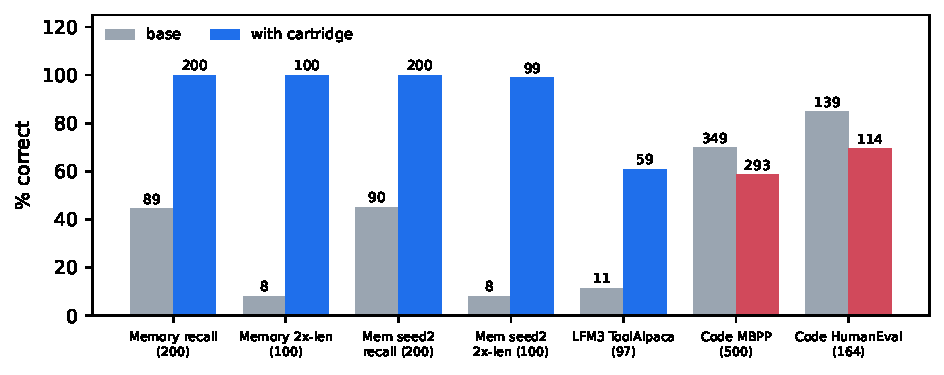
\includegraphics[width=\linewidth]{figures/fig5_other_cartridges.pdf}
\caption{Recall, LFM3 and code cartridges. Bars are \% correct; labels are counts. Red bars mark the code cartridge, which lowered accuracy.}
\label{fig:other}
\end{figure}

\subsection{Forgetting, perplexity and KL on the 27B cartridge}
\label{sec:forget}

We scored the run-1 27B ToolAlpaca cartridge on a 4-bit MLX build (mlx-community/Qwen3.8-27B-4bit, affine, group 64) against four off-task benchmarks, then WikiText-2 perplexity and forward KL, on an Apple-silicon Mac. An independent review re-derived the totals from the raw rows and matched them. The four tasks used the same seed-1234 item lists as a prior 0.5B run, but a 34.48\% evenly spaced subset of each list (1,528 of 4,439 items), because a full pass was estimated at 5.8 hours. The same items were scored with the mask off and on. Log-likelihood scoring was used throughout.

\begin{table}[h]
\centering
\small
\begin{tabular}{lrrrrrr}
\toprule
Task & $n$ / full & Base & On & Diff (pts) & Lost / gained & $p$ \\
\midrule
HellaSwag (acc\_norm) & 344 / 1,000 & 81.69\% & 81.40\% & $-0.29$ & 1 / 0 & 1.0 \\
MMLU (acc) & 344 / 1,000 & 80.81\% & 79.94\% & $-0.87$ & 5 / 2 & 0.45 \\
ARC-Challenge (acc) & 404 / 1,172 & 60.40\% & 59.65\% & $-0.74$ & 5 / 2 & 0.45 \\
WinoGrande (acc) & 436 / 1,267 & 78.44\% & 77.29\% & $-1.15$ & 8 / 3 & 0.23 \\
Mean of four tasks & 1,528 & 75.33\% & 74.57\% & $-0.76$ & 19 / 7 & -- \\
\bottomrule
\end{tabular}
\caption{Off-task scores for the 27B ToolAlpaca cartridge, 4-bit MLX. The mean difference has a paired bootstrap 95\% CI of $-1.41$ to $-0.13$ points. No single task is significant. Pooled over the 1,528 items, 19 are lost and 7 are gained (exact McNemar $p = 0.029$).}
\label{tab:forget}
\end{table}

All four tasks move down, each by less than 1.2 points, and the CI for the mean excludes zero. We read this as a small loss, about one point or less, that is probably real. Two caveats apply. First, the comparison rests on 26 flipped items. Second, log-likelihoods from this scorer can move by up to 1.0 nat when the same item is scored under a different batch shape (checked on 64 item-arms, all of which kept the same choice); both arms used identical batches, so the comparison is paired, but items with a narrow top-2 margin can flip for numerical reasons, and the CI covers item sampling only.

On the WikiText-2 raw test set (first 50,000 tokens, 48 windows of 1,024, 49,104 scored tokens, tokenized with the Qwen3.8 tokenizer) perplexity is 7.5956 with the mask off and 7.5712 with it on, a change of $-0.0243$ (95\% CI $-0.0378$ to $-0.0114$): slightly better with the cartridge, not worse. Mean forward KL per token, $\mathrm{KL}(\text{base}\,\Vert\,\text{on})$, is 0.00574 nats (window CI 0.00528 to 0.00624); the median, 95th percentile and maximum are 0.00257, 0.0171 and 4.57. Top-1 token agreement is 96.61\%. With the cartridge ejected, KL is exactly 0 on all 49,104 tokens and the log-probabilities match the loaded base. Prompt and decode throughput and peak memory are not measurably different with the mask on (median prompt 63.5 versus 63.7 tokens/s; decode 11.64 versus 11.73; peak MLX memory 18.26\,GB in both arms). This is one seed, one mask, one 4-bit scheme, and a 34\% subset; we have not yet run the same suite on the 9B cartridges.

\subsection{Cost}
\label{sec:cost}

Hugging Face Jobs billed the RTX PRO 6000 at \$2.75 per hour. A 400-step 9B ToolAlpaca run took 730 to 742\,s inside the container (download, Wanda calibration, base evaluation, training at 1.05 to 1.08\,s per step, and the masked evaluation), about \$0.60 billed. Measured job costs were \$0.96 and \$0.98 for the two recall runs, \$0.75 for code and \$0.22 for LFM3. The first 27B run took 26 minutes on two GPUs for \$2.38; the cartridge is 57.2\,MB compressed (28,730,353 of 5,704,253,440 gate-projection weights, 0.5037\%). A 9B cartridge is 20.2 to 20.5\,MB compressed, about 0.1 bits per masked weight and roughly 1/900 of the 19.3\,GB bf16 checkpoint.

\section{Related work}
\label{sec:related}

\paragraph{Deletion Tuning and mask learning.} Our work is a direct extension of Deletion Tuning \citep{lu2026deleting}, which itself relates to MaskLLM \citep{fang2024maskllm}, $L_0$ relaxations \citep{louizos2017l0} and Wanda \citep{sun2023wanda}. Learning binary masks over frozen weights to add tasks goes back at least to Piggyback \citep{mallya2018piggyback} and PackNet \citep{mallya2017packnet}; supermasks showed that masks alone can define a working network \citep{ramanujan2019hidden}, and Supermasks in Superposition stored many task masks over one fixed network and selected among them \citep{wortsman2020supsup}. The lottery ticket hypothesis \citep{frankle2018lottery} is the classical background. Our contribution is to test this per-task mask idea on current instruction-tuned LLMs with deletion-only masks, under quantization and composition, on small hardware.

\paragraph{Sparse and parameter-efficient fine-tuning.} Diff pruning \citep{guo2020diffpruning} and sparse fine-tuning \citep{ansell2021composable,ansell2024scaling} learn sparse value updates. Ansell et al.\ already composed sparse fine-tunings by addition for cross-lingual transfer \citep{ansell2021composable}, a close precedent for our union operator. SHiRA \citep{bhardwaj2024shira} trains a small fraction of weights directly to enable fast adapter switching and multi-adapter fusion on device, which is the deployment goal we share; unlike SHiRA, a cartridge writes no new values and stores one bit per masked weight. LoRA \citep{hu2021lora} and QLoRA \citep{dettmers2023qlora} are the standard alternatives. We have not yet run a LoRA baseline on the same data and steps.

\paragraph{Model merging and task localization.} Task arithmetic \citep{ilharco2022taskarith}, TIES-Merging \citep{yadav2023ties}, DARE \citep{yu2023dare} and model soups \citep{wortsman2022soups} combine fine-tuned weights. TALL-masks \citep{wang2024tall} learn binary masks that localize each task's information inside a merged task vector, and show that tasks occupy largely separate weights; our near-disjoint 7B masks are consistent with that picture. Knowledge-neuron and ROME-style editing \citep{dai2021knowledge,meng2022rome} localize facts in MLP weights; we plan to label the neurons that cartridges delete in the same spirit.

\paragraph{Name collision.} ``Cartridges'' is also the name of a method by Eyuboglu et al.\ \citep{eyuboglu2025cartridges} that trains small KV-cache representations of a long corpus through self-study. That work is unrelated in mechanism: it stores learned key--value states, while a skill cartridge is a weight-deletion mask. We use ``skill cartridge'' throughout to keep the two apart.

\section{Limitations}
\label{sec:limits}

\begin{itemize}
\item \textbf{Small test sets.} ToolAlpaca has 97 items. Per-model gains are highly significant, but between-model comparisons (9B versus 27B) are not tested for significance and differ by about 4 items.
\item \textbf{Confounded size comparison.} Qwen3.5-9B and the 27B model are different generations.
\item \textbf{Mostly in-distribution evaluation.} ToolAlpaca, Science and recall test the trained format. We have no broad out-of-distribution suite yet. Forgetting, perplexity and KL are reported for the 27B ToolAlpaca cartridge on a 34\% subset of four tasks in 4-bit (\S\ref{sec:forget}); the 9B cartridges have not been through the same suite.
\item \textbf{Format effects.} Part of every exact-match gain may be formatting. For LFM3 this is clearly a large part.
\item \textbf{Stacking was tested with two skills, on one 7B pair and one 9B pair.} Union kept 85\% and 87.5\% of the tool gain and 97.9\% and 90.8\% of the science gain, so interference is not zero. The 18-item 9B science drop from solo to union is not significant ($p = 0.105$). More than two cartridges are untested.
\item \textbf{The recall task is synthetic.}
\item \textbf{Code failed} with SFT on reference solutions; we do not know yet whether any deletion-only recipe works for code at this scale.
\item \textbf{No LoRA or full fine-tuning baseline} on our own tasks and models. \citep{lu2026deleting} provide those comparisons for their settings; we have not repeated them.
\item \textbf{4-bit results cover one quantization scheme} (MLX affine, 4 bits, group 64) and two models. On the 9B they cover three seeds and two application forms. GGUF and other schemes are untested.
\item \textbf{Single evaluation per condition} under greedy decoding; we did not sample.
\item \textbf{Model naming.} The 27B checkpoint is the Hugging Face model \texttt{Qwen/Qwen3.8-27B}, as recorded in the training job; the 4-bit build is \texttt{mlx-community/Qwen3.8-27B-4bit}.
\end{itemize}

\section{Ongoing work}
\label{sec:pending}

Neuron-level labels for the weights each cartridge deletes (using the Goodfire neuron atlas) are in progress and are not reported here.

\section{Conclusion}

Deletion Tuning masks work as skill cartridges on the kind of hardware a single person owns. A 9B model with a 21\,MB ToolAlpaca cartridge matched a 27B model with its own cartridge, the result held across three seeds with a shared core of deleted weights, the gain survived 4-bit quantization on all three seeds with a sub-millisecond live toggle, and two published 7B masks and two 9B masks stacked by union while keeping most of their gains (85\% and 87.5\% of the tool-use gain; 97.9\% and 90.8\% of the science gain). The method carried over to a hybrid convolution and attention architecture and to a recall skill. Code did not work with our recipe. On a 4-bit 27B build, four general-knowledge tasks dropped by a mean of 0.76 points. All of this rests on the method of Lu et al.\ \citep{lu2026deleting}, including the union operator they proposed; what we add is evidence that its masks can be treated as small, reproducible, composable files and served live from a quantized base.

\section*{Code and data availability}
The training scripts, the MLX loader (live apply and eject, bf16 and 4-bit), the evaluation and statistics code, and this paper's source and figures are at \url{https://github.com/austindixson/skill-cartridges} (MIT license). The cartridges reported here (three 9B ToolAlpaca seeds, the 9B Science cartridge, two 9B recall seeds, the 27B run-1 ToolAlpaca cartridge and the LFM3-1.7B ToolAlpaca cartridge) are at \url{https://huggingface.co/austindixson/skill-cartridges}, with each one's training summary and per-step metrics. The negative-result code cartridge is not distributed. ToolAlpaca and Science data and scorers are not redistributed; they are fetched from the SDFT authors' repository at the pinned commit given in Appendix~\ref{app:repro}.

\paragraph{Acknowledgments.} We thank Jack Lu, Zhenbang Yang, Mike Lasby, Tejas Pote, Yani Ioannou and Mengye Ren for releasing the Deletion Tuning code and masks, and Idan Shenfeld and coauthors for releasing the ToolAlpaca and Science data and evaluators. AI coding and writing assistants were used for experiment code, analysis and drafting; the author designed the study and verified all results.

\bibliographystyle{plainnat}
\bibliography{references}

\appendix
\section{Reproducibility details}
\label{app:repro}

\paragraph{Code.} Upstream \texttt{agentic-learning-ai-lab/deleting-weights} at commit \texttt{94f0340ebb574f95bb41d844165253a6785e215e}; SDFT data and scorers from \texttt{idanshen/Self-Distillation} at commit \texttt{d77573212fa0a3ae2eeb64b9b44db1c251f75e3e}. Training environment: torch 2.15.0 (CUDA 13.2 build), transformers 5.22.2, accelerate 1.15.0, datasets 5.2.0, safetensors 0.8.0, zstandard 0.25.0, flash-linear-attention 0.6.0. Inference on Apple silicon: MLX 0.32.4, mlx-lm 0.32.2. The training scripts, loader and cartridges are public at \url{https://github.com/austindixson/skill-cartridges} and \url{https://huggingface.co/austindixson/skill-cartridges}.

\paragraph{Hyperparameters.} Table~\ref{tab:hparams}.

\begin{table}[h]
\centering
\small
\begin{tabular}{ll}
\toprule
Setting & Value \\
\midrule
Target & every text-layer MLP gate projection (\texttt{gate\_proj}; \texttt{w1} for LFM3) \\
Steps / batch & 400 / 4 (27B run 1: 272 steps on 2 GPUs) \\
Optimizer & AdamW (fused), lr $5\times10^{-4}$, weight decay 0, clip 1.0 \\
Sharpness $\alpha$ & linear 100 $\to$ 1000 \\
Init & Wanda, $\eta = 1/2048$, prior strength 3, 256 calibration prompts \\
Regularizer & $\lambda = 10^{-5}\,(1 - t/T)$ \\
Loss & mean cross-entropy over answer tokens \\
Max length & 2048 (recall: 3072) \\
Seeds & ToolAlpaca 0, 2, 3; recall 0, 2; others 0 \\
Decoding & greedy, chat template, thinking off \\
Max new tokens & ToolAlpaca 1024, Science 2048, recall 64 \\
Hardware & 1$\times$ RTX PRO 6000 96\,GB (HF Jobs); MLX on Apple silicon (4-bit, stacking) \\
\bottomrule
\end{tabular}
\caption{Training and evaluation settings.}
\label{tab:hparams}
\end{table}

\paragraph{Overlap computation.} Masks are decoded from the upstream format; for every mask the decoded deleted count equals \texttt{zero\_params} in its config. Per-layer padding bits are excluded. Intersections are exact popcounts.

\paragraph{Per-run measurements (9B ToolAlpaca).} Seconds per step 1.050 / 1.057 / 1.080; training time 480 / 482 / 492\,s; in-container wall time 742 / 730 / 742\,s; final training cross-entropy 0.129 / 0.124 / 0.061; compressed mask 21,141,031 / 21,521,657 / 21,322,108 bytes; peak GPU memory 49.1\,GB.

\end{document}
